% Provenance (never printed): see sources/outline_sources.md (Year 1: compaction and
% cementation; basin types; subsidence, accommodation and sea-level change). Exercise and
% problem values in the Book 3 scratch calculator calc/ch23.py; figure data from
% figdata/bachelor-1/compaction.py and sea_level.py.
% Porosity and permeability are Book 1's (g6); diagenesis was met in Book 2 (g12) and is
% re-founded here; sedimentary basin was met in Book 2 (g11) and is re-founded here;
% isostasy and the equal-mass proposition are ch. 11's; passive margins and rifts ch. 13's;
% effective stress ch. 16's; the Last Glacial Maximum and glacial cycles Book 2's (g12).
% Pressure solution is defined in the Year 3 volume (deformation mechanisms): prose only.
% Backstripping, the stretching model and the comparison of basins are the Year 2 volume's.
\chapter{成岩作用与沉积盆地}\label{ch:b1:diagenesis-basins}

海滩沙是松散的：按体积计，其中一半是颗粒之间的水。埋深
三千米处，同样的沙子在钻探岩芯中以坚硬砂岩的形式重现，
颗粒被压紧，颗粒间的空隙大为缩小，
并被新生石英部分充填。从海滩到岩芯之间相隔数百万年，
沉积物在此期间被更多沉积物掩埋、挤压、加热，并浸泡在
水中，水溶解了一些\omterm{def:b1:rock-forming-minerals:mineral}{矿物}，又沉淀了另一些\omterm{def:b1:rock-forming-minerals:mineral}{矿物}。本章追踪这些变化，
随后回到能使沉积物堆积至千米厚的地方
即——\omterm{def:b1:diagenesis-basins:basin}{沉积盆地}——，以及为其提供空间的两个因素：
盆地底部的下沉，以及海平面的升降。

\begin{recall}
岩石的孔隙度是孔隙所占体积的比例，
渗透率衡量水流经孔隙的难易程度（第 1 册，六年级）。
当某一区域处于\omterm{def:b1:isostasy-gravity:isostasy}{地壳均衡}状态时，从地表向下直至\omterm{def:b1:isostasy-gravity:isostasy}{补偿深度}的每一竖直柱体
所含质量相同（\cref{prop:b1:isostasy-gravity:equal-mass}）。裂谷通过\omterm{def:b1:faults-folds-fabrics:fault-types}{正断层}张开，
\omterm{def:b1:rifts-ridges-margins:passive-margin}{被动大陆边缘}则是大陆的边缘，它们在裂谷
演化为洋盆时被遗留下来（\cref{ch:b1:rifts-ridges-margins}）。\omterm{def:b1:stress-strain-rheology:lithostatic}{有效应力}
是应力减去\omterm{def:b1:stress-strain-rheology:lithostatic}{孔隙流体压力}
（\cref{def:b1:stress-strain-rheology:lithostatic}）。末次冰期旋回
在约两万年前达到末次盛冰期（第 2 册，十二年级）。
砂岩、页岩及其环境见
\cref{ch:b1:clastic-sediments}；石灰岩、白垩、白云岩和\omterm{def:b1:chemical-biogenic-sediments:evaporite}{蒸发岩}见
\cref{ch:b1:chemical-biogenic-sediments}。
\end{recall}

\section{压实}\label{sec:b1:diagenesis-basins:compaction}

新沉积的沉积物是颗粒松散堆积而成、颗粒间充满水的集合体。
沉积之后、变质之前，只要沉积物仍处于\omterm{def:b1:layered-earth:layers}{地壳}上部数千米范围内的低温低压条件，
其间发生的一切变化
都同属于一类作用。

\begin{definition}[成岩作用]\label{def:b1:diagenesis-basins:diagenesis}
\emph{成岩作用}\index{成岩作用}是沉积物在沉积之后发生的
物理、化学和生物变化的总称，这些变化发生于上\omterm{def:b1:layered-earth:layers}{地壳}的
温度和压强条件下，且低于变质作用的温度和压强。它包括
\omterm{def:b1:diagenesis-basins:compaction}{压实}、胶结、颗粒溶解，以及一种\omterm{def:b1:rock-forming-minerals:mineral}{矿物}被另一种\omterm{def:b1:rock-forming-minerals:mineral}{矿物}取代；
这些作用共同使松散的沉积物变为
沉积岩。
\end{definition}

这些变化中的第一种是力学作用。每一新增沉积层都把
自身重量加到其下方各层上。颗粒被压紧、相互滑动并转动，
排列成更紧密的堆积；较软的颗粒（黏土片、岩屑、\omterm{def:b1:rock-forming-minerals:groups}{云母}）在较硬的颗粒之间弯曲，
颗粒间的水被挤出。
% ledger: og:diagenesis

\begin{definition}[压实、去压实]\label{def:b1:diagenesis-basins:compaction}
\emph{压实}\index{压实}是沉积物在上覆沉积物重量作用下体积减小的过程，
其方式包括颗粒排列趋于紧密、
孔隙水被排出，以及在较深处颗粒接触点的溶解。
\emph{去压实}\index{去压实}是一种计算，用于将埋藏岩层
恢复到较早、埋藏较浅时的厚度，
多数情况下即其刚沉积时位于地表的厚度。
\end{definition}

钻井中测得的孔隙度随深度减小，近地表处减小得很快，
之后则越来越慢。1930 年，L.~F. Athy 用指数函数拟合了这些数据，
此后该拟合便成为\omterm{def:b1:diagenesis-basins:compaction}{压实}研究的出发点。
% ledger: sc80:athy

\begin{proposition}[阿西定律]\label{prop:b1:diagenesis-basins:athy}
在由单一岩性构成的沉积物堆中，沉积物在自重作用下\omterm{def:b1:diagenesis-basins:compaction}{压实}，且其孔隙水
可自由排出时，地表以下深度 $z$ 处的孔隙度为
\[
  \varphi(z) = \varphi_0\, e^{-z/\lambda},
\]
其中 $\varphi_0$ 为地表孔隙度，$\lambda$ 为衰减长度，二者都取决于
岩性。这一关系即为\emph{阿西定律}\index{阿西定律}。
\end{proposition}
\admitted

该律是经验拟合，而非理论推论的结果。其参数
须逐一岩性地根据钻井孔隙度测定。
其数值见\cref{tab:b1:diagenesis-basins:athy}，随一项北海\omterm{def:b1:diagenesis-basins:subsidence}{沉降}研究发表，
被广泛用于校正\omterm{def:b1:diagenesis-basins:compaction}{压实}作用。页岩初始含水比砂岩多，
但失水的距离较短；白垩在地表处是三者中孔隙度最大的，
失水最快。在 \qty{3000}{m} 深处，此律给出的孔隙度为
\num{0.22}（砂岩）、\num{0.14}（页岩）和 \num{0.08}（白垩）（见下图）：
开篇所述的海滩沙已失去一半以上的孔隙。
% ledger: pybacktrack:compaction, sc80:north-sea

\begin{table}[htbp]
\centering
\begin{tabular}{lccc}
\hline
岩性 & 地表孔隙度 $\varphi_0$ & 衰减长度 $\lambda$（m） & 颗粒密度（\unit{kg.m^{-3}}） \\
\hline
页岩            & 0.63 & 1960 & 2700 \\
砂岩            & 0.49 & 3704 & 2650 \\
泥质砂岩        & 0.56 & 2564 & 2680 \\
白垩            & 0.70 & 1408 & 2710 \\
\hline
\end{tabular}
\caption{\omterm{prop:b1:diagenesis-basins:athy}{阿西定律}的参数及四种岩性的颗粒密度，
据 Sclater 和 Christie（1980），由开源回溯软件
pyBacktrack 列表给出。}
\label{tab:b1:diagenesis-basins:athy}
\end{table}
% ledger: pybacktrack:compaction

\omterm{def:b1:diagenesis-basins:compaction}{压实}作用只挤出水分，它既不增加颗粒，也不带走颗粒，
只要没有物质被溶解带走或作为\omterm{def:b1:diagenesis-basins:cement}{胶结物}带入。因此，
随地层柱埋藏需要追踪的量是地层柱中颗粒的
体积。

\begin{proposition}[地层的固体厚度]\label{prop:b1:diagenesis-basins:solid}
在\omterm{prop:b1:diagenesis-basins:athy}{阿西定律}下，深度介于 $z_1 < z_2$ 之间的地层，单位面积上所含颗粒的
体积等于其厚度
\[
  s = (z_2 - z_1) - \varphi_0 \lambda \left( e^{-z_1/\lambda} - e^{-z_2/\lambda} \right).
\]
若地层移至新的深度且颗粒既无损失也无增加，其新的顶面
$z_1'$ 与底面 $z_2'$ 满足 $s(z_1', z_2') = s(z_1, z_2)$，且对给定的
$z_1'$，该方程恰有一个解 $z_2'$。
\end{proposition}

\begin{proof}
厚度为 $\mathrm dz$ 的薄层位于深度 $z$ 处，其单位面积上所含颗粒的
体积为 $(1 - \varphi(z))\,\mathrm dz$。从 $z_1$ 积分至 $z_2$，
\[
  s = \int_{z_1}^{z_2} \bigl(1 - \varphi_0 e^{-z/\lambda}\bigr)\,\mathrm dz
    = (z_2 - z_1) - \varphi_0\lambda\left(e^{-z_1/\lambda} - e^{-z_2/\lambda}\right).
\]
固定顶面为 $z_1'$，函数 $f(b) = s(z_1', b)$ 的
导数为 $1 - \varphi(b) > 0$（孔隙度小于一），它
连续，在 $b = z_1'$ 处为零且无界增长，因此恰好一次取到
值 $s(z_1, z_2)$。
\end{proof}

\begin{method}[地层的去压实]\label{met:b1:diagenesis-basins:decompaction}
\begin{enumerate}
  \item 读取该地层今天的顶面 $z_1$ 与底面 $z_2$，以及其参数
        $\varphi_0$ 与 $\lambda$
        （见\cref{tab:b1:diagenesis-basins:athy}）。
  \item 用
        \cref{prop:b1:diagenesis-basins:solid}计算其固体厚度 $s$。
  \item 选取该地层在较早时刻顶面的深度 $z_1'$——取零即
        恢复到地表。
  \item 用牛顿法求解 $s(z_1', b) = s$，得到新的底面 $b$：
        取初值 $b_0 = z_1' + (z_2 - z_1)$，并重复
        \[
          b_{k+1} = b_k - \frac{s(z_1', b_k) - s}{1 - \varphi(b_k)}
        \]
        直至变化量小于所需精度；通常两三步
        即可满足要求。
  \item 该时刻地层的厚度为 $b - z_1'$，其平均
        孔隙度为 $1 - s/(b - z_1')$。
\end{enumerate}
\end{method}

取位于 \qty{3000}{m} 至 \qty{3500}{m} 之间的 \qty{500}{m} 页岩，
其中颗粒 \qty{440}{m}，水仅 \qty{60}{m}，平均孔隙度为
\num{0.12}。将其带回地表，同样的颗粒形成一层
\qty{891}{m} 厚的地层，其中一半为水（见下图）。埋藏页岩的厚度
仅略多于其原始沉积厚度的一半；从埋藏剖面读取的沉积速率
必须先经\omterm{def:b1:diagenesis-basins:compaction}{去压实}，方可与
今日测得的速率相比较。
% computed in figdata/bachelor-1/compaction.py; ledger: pybacktrack:compaction

\begin{omfigure}
\begin{tikzpicture}[font=\footnotesize]
\begin{axis}[name=phi, width=7.6cm, height=7.2cm, xmin=0, xmax=0.75, ymin=0, ymax=5000,
    y dir=reverse, xlabel={孔隙度 $\varphi$}, ylabel={深度 (m)},
    xtick={0,0.2,0.4,0.6}, ytick={0,1000,...,5000},
    legend style={at={(0.97,0.03)}, anchor=south east, font=\scriptsize, draw=none, fill=white, fill opacity=0.85, text opacity=1},
    legend cell align=left]
  \addplot[thick, omLithSand!50!black] table[x=phi_sand, y=z] {figdata/out/bachelor-1-compaction-curves.dat};
  \addplot[thick, omThm, densely dashed] table[x=phi_shale, y=z] {figdata/out/bachelor-1-compaction-curves.dat};
  \addplot[thick, omLithLime!50!black, dash dot] table[x=phi_chalk, y=z] {figdata/out/bachelor-1-compaction-curves.dat};
  \legend{砂岩, 页岩, 白垩}
  \draw[black!50, dotted] (axis cs:0,3000) -- (axis cs:0.75,3000);
\end{axis}
\begin{axis}[at={(phi.east)}, anchor=west, xshift=1.6cm, width=6.4cm, height=7.2cm,
    ybar stacked, bar width=1.1cm, ymin=0, ymax=1000, enlarge x limits=0.45,
    symbolic x coords={buried, surface}, xtick=data,
    xticklabels={{3000--3500 m 处}, {地表}},
    ylabel={地层厚度 (m)}, ytick={0,200,...,1000},
    legend style={at={(0.03,0.97)}, anchor=north west, font=\scriptsize, draw=none},
    legend cell align=left]
  \addplot[fill=omLithShale, draw=black!60] table[x=state, y=solid] {figdata/out/bachelor-1-compaction-demo.dat};
  \addplot[fill=omSea, draw=black!60] table[x=state, y=pore] {figdata/out/bachelor-1-compaction-demo.dat};
  \legend{颗粒, 孔隙水}
  \node[anchor=south] at (axis cs:buried,500) {\qty{500}{m}};
  \node[anchor=south] at (axis cs:surface,891) {\qty{891}{m}};
\end{axis}
\end{tikzpicture}

{\small 左图：\omterm{prop:b1:diagenesis-basins:athy}{阿西定律}给出的砂岩、页岩与白垩孔隙度随深度的变化，
参数取自\cref{tab:b1:diagenesis-basins:athy}。右图：
\qty{500}{m} 页岩，位于 \qty{3000}{m} 至 \qty{3500}{m} 之间，以及将同一
地层\omterm{def:b1:diagenesis-basins:compaction}{去压实}至地表的结果：颗粒（\qty{440}{m}）保留，水
则不予保留。}
\label{fig:b1:diagenesis-basins:compaction}
\end{omfigure}
% computed in figdata/bachelor-1/compaction.py; ledger: pybacktrack:compaction

\omterm{prop:b1:diagenesis-basins:athy}{阿西定律}只在水能排出时成立。\omterm{def:b1:diagenesis-basins:compaction}{压实}由\omterm{def:b1:stress-strain-rheology:lithostatic}{有效应力}驱动，
即上覆岩石重量减去孔隙中水的压强，
（见\cref{ch:b1:stress-strain-rheology}）。若厚层页岩埋藏得
快于其水分能够渗出的速度，水便承担一部分载荷，\omterm{def:b1:stress-strain-rheology:lithostatic}{孔隙流体压力}
升至高于静水压力，页岩保留的孔隙度相对其埋深过高，
此即超压，\omterm{def:b1:diagenesis-basins:compaction}{压实}校正时必须
对此予以考虑。
% ledger: sc80:north-sea

埋藏更深时，\omterm{def:b1:diagenesis-basins:compaction}{压实}转为化学作用。两颗石英颗粒经水膜相互挤压，
尤其是其间夹有黏土或\omterm{def:b1:rock-forming-minerals:groups}{云母}片时，
石英便在接触处溶解；二氧化硅
经水体短距离扩散，并沉淀于面向
开放孔隙的洁净石英表面上。颗粒相互穿插，溶解沿
表面集中发生，留下缝合线，即锯齿状的不溶残余物缝隙。这种压力
溶解（本科三年级分册将其视为一种变形机制）兼具两重身份：
既是\omterm{def:b1:diagenesis-basins:compaction}{压实}的最后阶段，也是砂岩中最常见\omterm{def:b1:diagenesis-basins:cement}{胶结物}的
来源。
% ledger: walderhaug:quartz, oye:quartz-cement

\section{胶结作用及其他变化}\label{sec:b1:diagenesis-basins:cementation}

仅靠\omterm{def:b1:diagenesis-basins:compaction}{压实}只能形成致密的沉积物，而非坚硬的岩石。颗粒
借生长于孔隙中的\omterm{def:b1:rock-forming-minerals:mineral}{矿物}胶结成岩。

\begin{definition}[胶结作用，胶结物]\label{def:b1:diagenesis-basins:cement}
\emph{胶结作用}\index{胶结作用}是\omterm{def:b1:rock-forming-minerals:mineral}{矿物}自孔隙水中析出的过程，
即沉积物孔隙中的孔隙水析出\omterm{def:b1:rock-forming-minerals:mineral}{矿物}，将颗粒胶结在一起，并
降低其孔隙度。析出的这些\omterm{def:b1:rock-forming-minerals:mineral}{矿物}构成
岩石的\emph{胶结物}\index{胶结物}；最常见的有石英、方解石、
铁的氧化物与\omterm{def:b1:weathering-clays:clay-mineral}{黏土矿物}。
\end{definition}

地下水以溶解态携带胶结\omterm{def:b1:rock-forming-minerals:mineral}{矿物}，
这些\omterm{def:b1:rock-forming-minerals:mineral}{矿物}的成分不必与颗粒相同。铁的氧化物包裹颗粒，
使岩石呈红色、褐色或黄色，科罗拉多高原的岩层即为例证；
方解石既胶结砂岩，也胶结石灰岩。
% ledger: og:diagenesis

石英是深埋砂岩的\omterm{def:b1:diagenesis-basins:cement}{胶结物}。它沿碎屑石英颗粒生长，
与之保持光学连续，以加大边的形式生长：在显微镜下，
颗粒与其加大边在\omterm{def:b1:field-lab-methods-1:microscope}{正交偏光}下同时变暗，
颗粒原有的轮廓只以一圈薄薄的尘土或黏土边缘显示
（见下图）。对北海与得克萨斯的砂岩作过详细研究，
加大边的氧同位素表明，\omterm{def:b1:diagenesis-basins:cement}{胶结作用}始于
\qtyrange{60}{80}{\celsius}，并持续到岩层达到其最大
埋藏温度；得克萨斯砂岩的石英\omterm{def:b1:diagenesis-basins:cement}{胶结物}占 \qtyrange{12}{18}{\percent}，北海砂岩
仅占 \qtyrange{2}{6}{\percent}，且二氧化硅大部分来自压力
溶解，发生于颗粒接触处。石英只在洁净的石英表面上生长，
因此颗粒上若包有一层黏土，供胶结的表面便减少，
深埋砂岩便可保留孔隙度。
% ledger: oye:quartz-cement, walderhaug:quartz

\begin{omfigure}
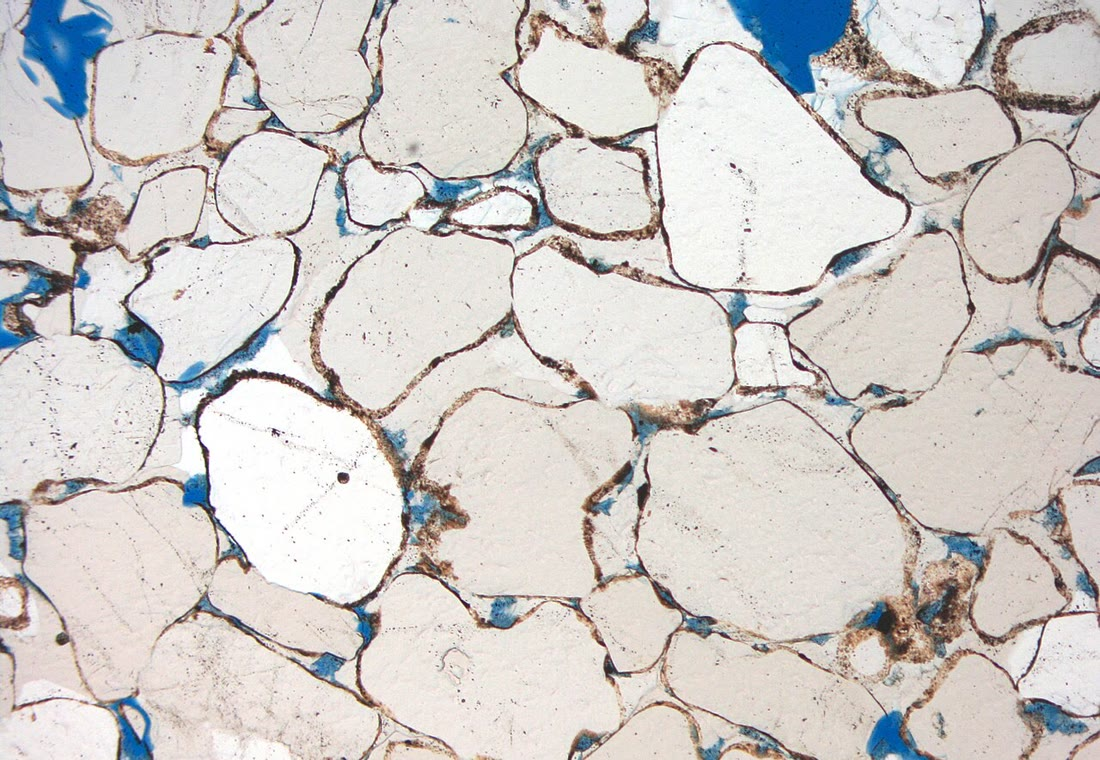
\includegraphics[width=0.62\linewidth]{images/book3/b1-quartz-overgrowths.jpg}

{\small 石英砂岩\omterm{def:b1:field-lab-methods-1:thin-section}{薄片}，取自美国纽约州的波茨坦砂岩（寒武纪），
\omterm{def:b1:field-lab-methods-1:microscope}{单偏光}下观察。圆化的碎屑颗粒
由暗色的尘土与黏土边缘勾勒轮廓；边缘之外清亮的石英
即为生长于颗粒上的\omterm{def:b1:diagenesis-basins:cement}{胶结物}，与之保持光学连续，直至
相邻加大边沿平直面相接。蓝色树脂充填
残存的孔隙。（M.~C.~Rygel，CC~BY-SA~4.0，经维基共享资源；
原图比例尺已裁剪。）}
\label{fig:b1:diagenesis-basins:overgrowths}
\end{omfigure}
% ledger: commons:potsdam

并非所有变化都会毁坏孔隙度。对某\omterm{def:b1:rock-forming-minerals:mineral}{矿物}未饱和的水会溶解该\omterm{def:b1:rock-forming-minerals:mineral}{矿物}：
\omterm{def:b1:rock-forming-minerals:groups}{长石}与碳酸盐颗粒，以及早先的碳酸盐\omterm{def:b1:diagenesis-basins:cement}{胶结物}，都可能被溶去，
留下次生孔隙，
其形状与所取代的颗粒一致。\omterm{def:b1:weathering-clays:clay-mineral}{黏土矿物}随后又在孔隙中生长，
或作为颗粒上的包膜，或作为充填孔隙的晶体，并缩窄孔道，
从而降低渗透率。沉积物中的\omterm{def:b1:rock-forming-minerals:mineral}{矿物}也会改变：
贝壳与\omterm{def:b1:chemical-biogenic-sediments:factory}{碳酸盐工厂}中的文石，会转变为地表稳定的方解石，
而在含镁水中，方解石可能
转变为白云石。
% ledger: og:diagenesis

方解石被白云石取代，即白云石化，是一个与水中
镁发生的反应，
\[
  \ce{2 CaCO3 + Mg^2+ -> CaMg(CO3)2 + Ca^2+},
\]
并使固相体积发生变化。

\begin{proposition}[白云石化形成孔隙]\label{prop:b1:diagenesis-basins:dolomite}
若密度为 $\rho_c$ 的两摩尔方解石被一摩尔
密度为 $\rho_d$ 的白云石所取代，则固相体积减小的比例为
\[
  1 - \frac{M_d/\rho_d}{2M_c/\rho_c},
\]
其中 $M_c$ 与 $M_d$ 为摩尔质量。取 $\rho_c = \qty{2.71}{g.cm^{-3}}$
$\rho_d = \qty{2.84}{g.cm^{-3}}$，此比例为 \qty{12.1}{\percent}。
\end{proposition}

\begin{proof}
\omterm{def:b1:rock-forming-minerals:mineral}{矿物}的摩尔体积等于其摩尔质量除以其密度。两摩尔
方解石占据 $2M_c/\rho_c$，一摩尔白云石占据 $M_d/\rho_d$；损失的
比例即一减去二者之比。取 $M_c = \qty{100.09}{g.mol^{-1}}$
，$M_d = \qty{184.40}{g.mol^{-1}}$，二者体积分别为
$2\times\qty{36.93}{cm^3} = \qty{73.86}{cm^3}$ 与 \qty{64.93}{cm^3}，且
$1 - 64.93/73.86 = \num{0.121}$。
\end{proof}

若岩石的外部体积不变，则损失的固体即为增加的孔隙空间：
孔隙度为 \num{0.10} 的石灰岩若按摩尔对摩尔被白云石取代，其孔隙度
约为 \num{0.21}。该反应需要大量的镁，
海水中的镁含量约为每千克 \qty{1.28}{g}；在
卤水或海水长期流经岩石的条件下，该反应更易发生
（见\cref{exo:b1:diagenesis-basins:12}）。
% ledger: hom:calcite, webmineral:others, teos10:reference-composition, teos10:reference-salinity

\omterm{def:b1:diagenesis-basins:diagenesis}{成岩作用}沿沉积物的历史展开。刚沉积之后，近地表处，
孔隙水仍是海水、湖水或雨水：
沉积物被生物扰动，在海底或土壤中早期即发生胶结，并
文石转变为方解石。随埋藏加深与升温，\omterm{def:b1:diagenesis-basins:compaction}{压实}、
压力溶解及石英胶结逐渐占据主导。若盆地
此后抬升并遭受侵蚀，地表淡水重新流入
岩石，再次溶解碳酸盐与\omterm{def:b1:rock-forming-minerals:groups}{长石}。\omterm{def:b1:field-lab-methods-1:thin-section}{薄片}记录了
这些事件的先后：充填被溶去颗粒所留孔隙的\omterm{def:b1:diagenesis-basins:cement}{胶结物}，
比溶解作用年轻；被\omterm{def:b1:diagenesis-basins:compaction}{压实}作用破坏的加大边，
则比\omterm{def:b1:diagenesis-basins:compaction}{压实}作用古老。

\section{沉积盆地}\label{sec:b1:diagenesis-basins:basins}

厚达数千米的沉积物，只在地表持续下沉之处才会堆积。

\begin{definition}[沉积盆地]\label{def:b1:diagenesis-basins:basin}
\emph{沉积盆地}\index{沉积盆地}是指地表的某一区域，
\omterm{def:b1:layered-earth:layers}{地壳}在该处长期\omterm{def:b1:diagenesis-basins:subsidence}{沉降}，时间跨度为数百万至数亿年，
且由此形成的空间已被沉积物充填，
沉积物厚度从数百米到数千米不等。
\end{definition}

\begin{definition}[沉降，构造沉降]\label{def:b1:diagenesis-basins:subsidence}
盆地的\emph{沉降}\index{沉降}是指其基底的向下运动，
基底即沉积物所覆盖的面，沉降以相对于固定
参照面（如地心）来度量。其\emph{构造沉降}\index{构造沉降}
是由形成盆地的构造过程引起的部分，
有别于充填盆地的沉积物与水的重量
所引起的额外下沉；它以仅由水负荷时
基底本应发生的沉降量来度量。
\end{definition}

使盆地底板下沉的，是盆地在板块中的位置
（见下图）。

\begin{description}
  \item[裂谷盆地。] \omterm{def:b1:faults-folds-fabrics:fault-types}{正断层}拉伸\omterm{def:b1:layered-earth:layers}{地壳}，断块在其间下陷
        （见\cref{ch:b1:rifts-ridges-margins}）。盆地狭窄而不对称，
        \omterm{def:b1:rifts-ridges-margins:rift}{半地堑}沿边界断层一侧充填最快。北海的油田
        位于维京\omterm{def:b1:rifts-ridges-margins:rift}{地堑}与中央\omterm{def:b1:rifts-ridges-margins:rift}{地堑}的构造之中，
        被较新的沉积物掩埋。伸展停止后，
        变薄受热的\omterm{def:b1:layered-earth:lithosphere}{岩石圈}冷却、收缩并继续
        缓慢下沉，历时数千万年。北海中部，
        其最后一次大规模伸展结束于白垩纪中期，随后\omterm{def:b1:diagenesis-basins:subsidence}{沉降}成一个
        宽阔的碟形盆地，依次被白垩、砂岩
        以及第三纪大部分时间里的页岩与泥岩充填；其基底
        仅受水的负荷，中部本应下沉 \qtyrange{1100}{1400}{m}
        。
  \item[\omterm{def:b1:rifts-ridges-margins:passive-margin}{被动大陆边缘}。] 裂谷演化为洋盆之后，同样的冷却作用
        使每一侧边缘在破裂后下沉，朝向洋一侧增厚的沉积楔
        在老裂谷盆地之上逐渐发育。
  \item[前陆盆地。] 在逆冲带前方，叠置逆冲岩片的重量
        通过\omterm{def:b1:isostasy-gravity:isostasy}{地壳均衡}使\omterm{def:b1:layered-earth:lithosphere}{岩石圈}向下弯曲，形成盆地
        其最深处紧邻造山带，由造山带剥蚀的碎屑充填。
        加拿大西部的白垩纪岩层大部分
        沉积于落基山脉前方的此类盆地中。
  \item[克拉通内盆地。] 古老大陆内部，远离任何板块边界处，
        宽广的圆形或椭圆形区域缓慢下沉了极长时间。
        巴黎盆地即是此类构造凹陷的中心，
        位于古老地块布列塔尼、中央高原与
        孚日山脉及阿登高原之间。
  \item[走滑盆地。] \omterm{def:b1:faults-folds-fabrics:fault-types}{走滑断层}在使两盘相互拉开的方向上转折
        ——即释放弯曲——处，两条断层分支之间的一块平行四边形\omterm{def:b1:layered-earth:layers}{地壳}
        发生\omterm{def:b1:diagenesis-basins:subsidence}{沉降}，形成拉分盆地，
        如沿圣安德烈亚斯断层系分布的洛杉矶地区盆地。
\end{description}
% ledger: ws:basins, sc80:north-sea, britannica:paris-basin

各类盆地中\omterm{def:b1:layered-earth:lithosphere}{岩石圈}为何下沉、以何种速率下沉，以及
各类盆地如何比较，属于本科二年级分册的内容；此处只按
盆地所在位置及其充填物的形态加以区分。

\begin{omfigure}
\begin{tikzpicture}[font=\scriptsize, line join=round]
% (a) rift: a half-graben
\begin{scope}
  \fill[lith granite] (0,0) -- (0,1.6) -- (1.4,1.6) -- (2.2,0.2) -- (5.0,1.0) -- (5.0,0) -- cycle;
  \fill[lith shale] (1.4,1.6) -- (2.2,0.2) -- (5.0,1.0) -- (5.0,1.6) -- cycle;
  \fill[lith sandstone] (1.4,1.6) -- (1.75,0.99) -- (5.0,1.25) -- (5.0,1.6) -- cycle;
  \draw[normal fault, thick] (1.4,1.6) -- (2.3,0.0);
  \draw[black!70] (0,1.6) -- (5.0,1.6);
  \node[anchor=south west] at (0,1.65) {(a) 裂谷：半地堑};
  \node[fill=white, fill opacity=0.8, text opacity=1, inner sep=1pt] at (3.9,0.3) {基底};
  \node[fill=white, fill opacity=0.8, text opacity=1, inner sep=1pt] at (0.65,0.8) {下盘};
\end{scope}
% (b) passive margin: a seaward-thickening wedge over thinned crust
\begin{scope}[xshift=6.6cm]
  \fill[lith sea] (2.0,1.6) -- (5.0,1.6) -- (5.0,0.75) -- (3.6,0.95) -- cycle;
  \fill[lith granite] (0,0) -- (0,1.2) -- (2.0,1.0) -- (3.6,0.35) -- (5.0,0.05) -- (5.0,0) -- cycle;
  \fill[lith shale] (0,1.2) -- (2.0,1.0) -- (3.6,0.35) -- (5.0,0.05) -- (5.0,0.75) -- (3.6,0.95) -- (2.0,1.6) -- (0,1.6) -- cycle;
  \draw[black!70] (0,1.6) -- (2.0,1.6) -- (3.6,0.95) -- (5.0,0.75);
  \draw[blue!60!black, thick] (2.0,1.6) -- (5.0,1.6);
  \node[anchor=south west] at (0,1.65) {(b) 被动大陆边缘};
  \node[fill=white, fill opacity=0.8, text opacity=1, inner sep=1pt] at (1.0,0.45) {减薄的陆壳};
  \node[anchor=north east] at (5.0,1.58) {海洋};
\end{scope}
% (c) foreland basin: asymmetric, deepest against the thrust belt
\begin{scope}[yshift=-3.3cm]
  \fill[lith granite] (0,0) -- (0,0.55) -- (5.0,1.35) -- (5.0,0) -- cycle;
  \fill[lith sandstone] (0,0.55) -- (5.0,1.35) -- (5.0,1.6) -- (0,1.6) -- cycle;
  \fill[lith conglomerate] (1.0,1.6) -- (3.6,1.6) -- (1.0,1.0) -- cycle;
  \fill[omLithSchist, draw=black!70] (0,0.95) -- (1.9,1.6) -- (1.3,1.95) -- (0.4,2.25) -- (0,2.3) -- cycle;
  \draw[thrust fault] (0,0.95) -- (1.9,1.6);
  \draw[thrust fault] (0,1.55) -- (1.15,1.95);
  \draw[black!70] (1.9,1.6) -- (5.0,1.6);
  \node[anchor=south west] at (2.0,1.65) {(c) 前陆盆地};
  \node[anchor=south west, inner sep=1pt] at (0.25,2.3) {逆冲带};
  \node[fill=white, fill opacity=0.8, text opacity=1, inner sep=1pt] at (3.9,0.35) {基底};
\end{scope}
% (d) intracratonic basin: a broad sag, layers thickening to the centre
\begin{scope}[xshift=6.6cm, yshift=-3.3cm]
  \fill[lith granite] (0,0) -- (0,1.5) .. controls (1.6,1.1) and (2.0,0.3) .. (2.5,0.3) .. controls (3.0,0.3) and (3.4,1.1) .. (5.0,1.5) -- (5.0,0) -- cycle;
  \fill[lith limestone] (0,1.5) .. controls (1.6,1.1) and (2.0,0.3) .. (2.5,0.3) .. controls (3.0,0.3) and (3.4,1.1) .. (5.0,1.5) -- (5.0,1.6) -- (0,1.6) -- cycle;
  \fill[lith shale] (0.6,1.6) .. controls (1.6,1.35) and (2.1,0.85) .. (2.5,0.85) .. controls (2.9,0.85) and (3.4,1.35) .. (4.4,1.6) -- cycle;
  \fill[lith sandstone] (1.3,1.6) .. controls (1.9,1.5) and (2.2,1.3) .. (2.5,1.3) .. controls (2.8,1.3) and (3.1,1.5) .. (3.7,1.6) -- cycle;
  \draw[black!70] (0,1.6) -- (5.0,1.6);
  \node[anchor=south west] at (0,1.65) {(d) 克拉通内盆地};
  \node[fill=white, fill opacity=0.8, text opacity=1, inner sep=1pt] at (4.2,0.4) {基底};
\end{scope}
\end{tikzpicture}

{\small 四类\omterm{def:b1:diagenesis-basins:basin}{沉积盆地}剖面示意（示意图，非按比例绘制；
垂向比例已放大）。(a)~裂谷：充填物
沿\omterm{def:b1:rifts-ridges-margins:rift}{半地堑}的边界断层一侧增厚。(b)~\omterm{def:b1:rifts-ridges-margins:passive-margin}{被动大陆边缘}：
沉积楔朝洋方向增厚，覆于减薄的陆壳之上。(c)~前陆盆地，
最深处紧邻逆冲带，其重量使盆地向下弯曲，并由
逆冲带的碎屑充填，靠近造山带处粒度最粗（砾岩）；造山带
逆掩于本盆地的边缘之上。(d)~克拉通内盆地：宽缓的凹陷，
层位向中心增厚。}
\label{fig:b1:diagenesis-basins:types}
\end{omfigure}

\begin{inthefield}[盆地是如何被认识的]
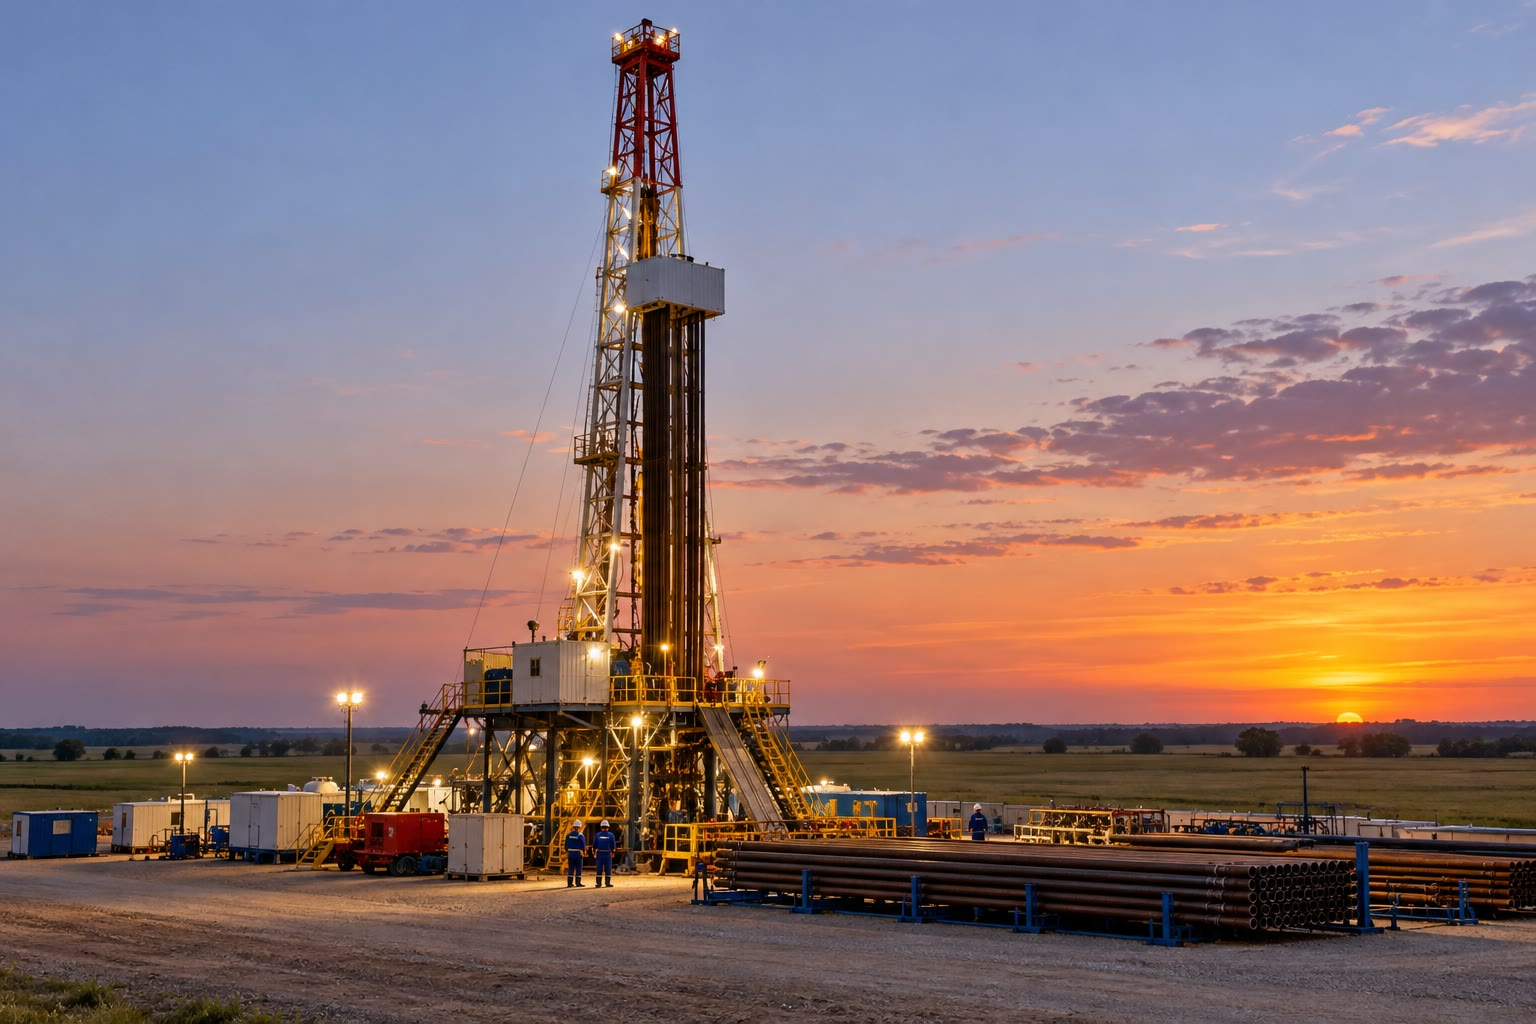
\includegraphics[width=0.3\linewidth]{images/book3/ai/b1-drilling-rig.jpg}\hfill
\begin{minipage}[b]{0.67\linewidth}
关于盆地深部充填物的认识，几乎全部来自
对石油、天然气和水的勘探。地震反射测量可在
数千平方千米范围内成像其地层与断层；井只能在一点取样。钻井
返回钻头切下的岩屑，间隔取得岩芯，还有
井周岩石物理性质的连续测井曲线，由此可逐米读出
孔隙度。\omterm{prop:b1:diagenesis-basins:athy}{阿西定律}的孔隙度–深度曲线，以及盆地的
\omterm{def:b1:diagenesis-basins:subsidence}{沉降}史，最初都是由此类钻井资料建立的。
\end{minipage}

\smallskip
{\small 黄昏时分的陆上钻机，前景处钻杆堆放在钻杆架上（AI
插图）。}
\end{inthefield}
% ledger: sc80:north-sea

\section{沉降、可容纳空间与海平面}\label{sec:b1:diagenesis-basins:accommodation}

沉积物只有在其会被继续搬运走的水平面以下
存在容纳空间时才能堆积。在海中，该水平面
接近海平面，而空间的大小取决于两种运动：盆底的运动与海面的运动。

\begin{definition}[可容纳空间]\label{def:b1:diagenesis-basins:accommodation}
称盆地中某点的\emph{可容纳空间}\index{可容纳空间}为该点可供沉积物堆积的
空间，即沉积物顶面至海平面的竖直距离（海平面是
海相沉积的基准面）。某一时间段内新产生的
可容纳空间，即附着于基底的基准面至海平面距离的
增量。
\end{definition}

\begin{definition}[全球海平面变化，相对海平面]\label{def:b1:diagenesis-basins:eustasy}
\emph{全球海平面变化}\index{全球海平面变化}是世界大洋水面高度
相对于固定参照（地心）的变化，由海洋中水的体积
或洋盆容积的
变化引起，在各处相同。\emph{相对海
平面}\index{相对海平面}指某地海面高出该处基底
所附基准面的高度；它随全球海平面变化
与地面的竖向运动而改变。
\end{definition}

\begin{proposition}[可容纳空间的收支]\label{prop:b1:diagenesis-basins:budget}
在某一时间段内，设 $\Delta E$ 为全球海平面的上升量，$S$
为基底的\omterm{def:b1:diagenesis-basins:subsidence}{沉降}量（二者的正方向：对海面向上，对海底
即向下）。新产生的\omterm{def:b1:diagenesis-basins:accommodation}{可容纳空间}为
\[
  \Delta A = \Delta E + S ,
\]
它由基准面以上新增的沉积物厚度 
$\Delta T$ 与水深的增加 $\Delta W$ 分担：
$\Delta E + S = \Delta T + \Delta W$。
\end{proposition}

\begin{proof}
以固定参照面为基准量取高度。设 $e$ 为海面高度，
$b$ 为基准面的高度，$T$ 为基准面之上沉积物的厚度，
并设 $W$ 为沉积物之上的水深，于是 $e = b + T + W$。\omterm{def:b1:diagenesis-basins:eustasy}{相对海平面}
为 $R = e - b = T + W$。在该时间段内，$\Delta e =
\Delta E$，且 $\Delta b = -S$，故 $\Delta R = \Delta E + S$；又 $\Delta R =
\Delta T + \Delta W$。
\end{proof}

水深保持不变（$\Delta W = 0$）的海底，其填充速度恰好与
\omterm{def:b1:diagenesis-basins:accommodation}{可容纳空间}的产生速度相同；水深变浅的海底被填充得更快，海岸线
向海推进；水深加大的海底则沉积不足。$\Delta T$ 为
基准面以上整个沉积层的厚度变化：它计入新沉积的
沉积物，并扣除下方较老沉积物在\omterm{def:b1:diagenesis-basins:compaction}{压实}过程中的减薄量，因此
\omterm{def:b1:diagenesis-basins:compaction}{压实}作用本身即可为更多沉积物腾出空间（见下图）。

\begin{omfigure}
\begin{tikzpicture}[font=\footnotesize, >=Stealth]
\def\col#1#2#3#4#5{% x, datum, sediment top, sea, label
  \fill[lith granite] (#1,0.2) rectangle ++(1.4,#2-0.2);
  \fill[lith shale] (#1,#2) rectangle ++(1.4,#3-#2);
  \fill[lith sea] (#1,#3) rectangle ++(1.4,#4-#3);
  \draw[black!70] (#1,#2) -- ++(1.4,0);
  \draw[blue!60!black, thick] (#1-0.2,#4) -- ++(1.8,0);
  \node[anchor=north] at (#1+0.7,0.15) {#5};}
\draw[black!60, dash dot] (-0.6,0.9) -- (8.6,0.9) node[anchor=west, align=left] {固定 \\ 参照面};
\col{0}{1.5}{3.0}{3.6}{时刻 $t_1$}
\col{4.4}{1.0}{3.4}{3.9}{时刻 $t_2$}
% eustasy
\draw[<->, omThm] (3.0,0.9) -- (3.0,3.6) node[midway, fill=white, inner sep=1pt] {$e_1$};
\draw[<->, omThm] (7.4,0.9) -- (7.4,3.9) node[midway, fill=white, inner sep=1pt] {$e_2$};
% subsidence of the datum
\draw[dashed, black!60] (1.4,1.5) -- (4.4,1.5);
\draw[->, thick] (4.2,1.5) -- (4.2,1.0) node[midway, anchor=east] {$S$};
% relative sea level
\draw[<->] (-0.35,1.5) -- (-0.35,3.6) node[midway, anchor=east] {$R_1$};
\draw[<->] (6.05,1.0) -- (6.05,3.9) node[midway, anchor=west] {$R_2$};
\node[anchor=west] at (1.5,2.25) {$T_1$};
\node[anchor=west] at (1.5,3.3) {$W_1$};
\node at (5.1,2.2) {$T_2$};
\node at (5.1,3.65) {$W_2$};
\node[anchor=south, align=center, blue!60!black] at (5.1,3.95) {海平面};
\node[anchor=west, align=left, font=\scriptsize] at (8.6,2.4) {$R = e - b = T + W$\\[2pt] $\Delta R = \Delta E + S$\\ $\phantom{\Delta R} = \Delta T + \Delta W$};
\end{tikzpicture}

{\small 同一地点在两个时刻的\omterm{def:b1:diagenesis-basins:accommodation}{可容纳空间}（示意）。$t_1$ 与
$t_2$ 之间，海平面相对固定参照面上升 $\Delta E = e_2 - e_1$，
基底下沉 $S$：\omterm{def:b1:diagenesis-basins:eustasy}{相对海平面} $R$ 增加 $\Delta E + S$，
即新产生的\omterm{def:b1:diagenesis-basins:accommodation}{可容纳空间}，由更多沉积物（$T_2 > T_1$）
与水深变化（此处为轻微变浅，$W_2 < W_1$）共同分担。}
\label{fig:b1:diagenesis-basins:accommodation}
\end{omfigure}

盆地的下沉并非仅由\omterm{def:b1:diagenesis-basins:subsidence}{构造沉降}引起：充填其中的
沉积物本身即是一种负荷，使\omterm{def:b1:layered-earth:lithosphere}{岩石圈}在其下进一步下沉。

\begin{proposition}[沉积负荷加剧沉降]\label{prop:b1:diagenesis-basins:loading}
在密度为 $\rho_m$ 的\omterm{def:b1:layered-earth:layers}{地幔}之上的局地（艾里）均衡中，若某盆地的
基底仅受密度为 $\rho_w$ 的水负荷时，将位于
海平面以下深度 $Y$ 处。若以平均密度为 $\rho_s$ 的沉积物充填至海平面，则其
厚度为
\[
  h = Y\,\frac{\rho_m - \rho_w}{\rho_m - \rho_s}
\]
沉积物。若在陆上，充填至周围地面高度，上方为空气，
则系数为 $\rho_m/(\rho_m - \rho_s)$。
\end{proposition}

\begin{proof}
比较两个柱体，二者\omterm{def:b1:layered-earth:lithosphere}{岩石圈}相同，单位面积质量为 $M$，
厚度为 $L$，二者均算至其下的\omterm{def:b1:isostasy-gravity:isostasy}{补偿深度} $z_c$。水负荷
柱体的质量为 $\rho_w Y + M + \rho_m(z_c - Y - L)$；沉积物充填的
柱体质量为 $\rho_s h + M + \rho_m(z_c - h - L)$。
由\cref{prop:b1:isostasy-gravity:equal-mass}可知两柱体质量相等，因此
$\rho_w Y - \rho_m Y = \rho_s h - \rho_m h$，即 $h(\rho_m - \rho_s) =
Y(\rho_m - \rho_w)$。若以空气代替水，则 $\rho_w$ 取零。
\end{proof}

取 $\rho_m = \qty{3300}{kg.m^{-3}}$，$\rho_w = \qty{1030}{kg.m^{-3}}$，且
沉积物平均密度为 \qty{2300}{kg.m^{-3}}，则系数为
$2270/1000 = \num{2.27}$：若某盆地的\omterm{def:b1:diagenesis-basins:subsidence}{构造沉降}可容纳
\qty{1}{km} 深的水，则可充填 \qty{2.27}{km} 厚的沉积物。若在陆上，系数将
为 $3300/1000 = \num{3.3}$。充填物的密度并非恒定，随沉积物\omterm{def:b1:diagenesis-basins:compaction}{压实}而增大，
系数也随之增大，因此要将沉积物厚度换算为\omterm{def:b1:diagenesis-basins:subsidence}{构造沉降}，
需对每一层作\omterm{def:b1:diagenesis-basins:compaction}{去压实}，
逐时间步进行。该方法即回剥法，属于本科二年级
分册。

海平面本身远非固定不变。末次盛冰期时，冰盖
覆盖了北美大部分地区与欧洲北部，而被封存于其中的水
原取自海洋。若扣除固体地球对
冰与水负荷变化的响应，则古海岸线的观测给出
于约 \num{30000} 年前，海平面快速下降约 \qty{40}{m}，
随后缓慢下降，于 \qtyrange{29}{21}{\ka} 间降至比今日低 \qty{134}{m}；
当时陆地冰量比今日多约 \qty{52e6}{km^3}。常被引用的
\qty{125}{m} 这一数值偏小，因其通常未对
这些均衡效应作修正。去冰期主要发生于约 \qty{16.5}{\ka}
至 \qty{8.2}{\ka} 之间，平均每千年上升 \qty{12}{m}，并且
在 \qty{14.5}{\ka} 至 \qty{14.0}{\ka} 之间，速率达每年 \qty{40}{mm} 或更高。
% ledger: lambeck:lgm, lambeck:deglaciation

更早的低海面期由深海
岩芯中有孔虫的氧同位素读取，它们记录了陆上冰的体积。将此类
重建结果叠加：近 \num{430000} 年取七组，近
\num{800000} 年取五组，叠加以平均掉各自的误差；经标定至全新世与
末次冰期低海面后，该叠加序列的不确定度为
\qtyrange{9}{12}{m}（见下图）。它将冰期旋回表现为锯齿形：
海平面缓慢下降，每次以快速上升收尾——在
近 \num{800000} 年间，有五次上升超过 \qty{100}{m}，历时不足 \num{20000}
年。这一尺度的\omterm{def:b1:diagenesis-basins:eustasy}{全球海平面变化}使海岸线在
大陆架上来回移动。
% ledger: spratt:stack, data:b3-sealevel-stack

\begin{omfigure}
\begin{tikzpicture}[font=\footnotesize]
\begin{axis}[width=16cm, height=4.8cm, xmin=0, xmax=800, ymin=-150, ymax=40,
    x dir=reverse, xlabel={年龄（距今千年）}, xlabel style={yshift=2pt},
    ylabel={海平面 (m)}, ytick={-150,-100,-50,0},
    title={(a) 近 \num{800000} 年（五组记录）}, title style={font=\footnotesize},
    axis on top]
  \addplot[draw=none, name path=hi] table[x=age, y=hi] {figdata/out/bachelor-1-sea_level-long.dat};
  \addplot[draw=none, name path=lo] table[x=age, y=lo] {figdata/out/bachelor-1-sea_level-long.dat};
  \addplot[omThm!25] fill between[of=hi and lo];
  \addplot[thin, omThm] table[x=age, y=sl] {figdata/out/bachelor-1-sea_level-long.dat};
  \draw[black!50, densely dotted] (axis cs:0,0) -- (axis cs:800,0);
\end{axis}
\end{tikzpicture}

\medskip
\begin{tikzpicture}[font=\footnotesize]
\begin{axis}[width=16cm, height=4.8cm,
    xmin=0, xmax=140, ymin=-160, ymax=40, x dir=reverse,
    xlabel={年龄（距今千年）}, ylabel={海平面 (m)},
    ytick={-150,-100,-50,0},
    title={(b) 近 \num{140000} 年（七组记录）}, title style={font=\footnotesize},
    axis on top]
  \addplot[draw=none, name path=hi] table[x=age, y=hi] {figdata/out/bachelor-1-sea_level-short.dat};
  \addplot[draw=none, name path=lo] table[x=age, y=lo] {figdata/out/bachelor-1-sea_level-short.dat};
  \addplot[omThm!25] fill between[of=hi and lo];
  \addplot[thick, omThm] table[x=age, y=sl] {figdata/out/bachelor-1-sea_level-short.dat};
  \draw[black!50, densely dotted] (axis cs:0,0) -- (axis cs:140,0);
  \addplot[only marks, mark=*, mark size=1.6pt, black] coordinates {(21,-134)};
  \draw[black!60, thin] (axis cs:21,-131) -- (axis cs:21,-46);
  \node[anchor=south, font=\scriptsize, fill=white, inner sep=1pt] at (axis cs:36,-46) {\qty{21}{\ka} 时古海岸线所示 \qty{-134}{m}（Lambeck et al.\ 2014）};
\end{axis}
\end{tikzpicture}

{\small 相对今日的全球海平面，取自 Spratt 与
Lisiecki (2016)：五组重建的第一主成分，取自
深海岩芯，覆盖近 \num{800000} 年（a），另取七组覆盖近
\num{140000} 年（b），并附一倍标准差范围。叠加序列的最低值
为 \qty{-130}{m}，出现于 \qty{24}{\ka}，位于由古海岸线得出的
\qty{-134}{m}（图中的点）的范围之内；末次间冰期
约在 \qty{121}{\ka} 时高于今日约 \qty{3}{m}。数据：NOAA NCEI World Data
Service for Paleoclimatology.}
\label{fig:b1:diagenesis-basins:sea-level}
\end{omfigure}
% computed in figdata/bachelor-1/sea_level.py; ledger: data:b3-sealevel-stack, spratt:stack, lambeck:lgm

在盆地的整个演化过程中，此类摆动持续时间很短。冰期时海平面下降超过
\qty{100}{m}，历时仅数万年，与\omterm{def:b1:diagenesis-basins:subsidence}{构造沉降}相比既快又大，
而\omterm{def:b1:diagenesis-basins:subsidence}{构造沉降}须经数千万年才累积达一千米或更多；
但冰期摆动的幅度大致限于
约 \qty{150}{m} 之内，因此在盆地厚厚的充填物中，\omterm{def:b1:diagenesis-basins:subsidence}{沉降}占据了
大部分\omterm{def:b1:diagenesis-basins:accommodation}{可容纳空间}，\omterm{def:b1:diagenesis-basins:eustasy}{全球海平面变化}则决定其地层的节奏。
% ledger: data:b3-sealevel-stack, sc80:north-sea

\section{练习}

\begin{exercise}[$\star$]\label{exo:b1:diagenesis-basins:1}
利用 \cref{tab:b1:diagenesis-basins:athy} 中的参数，计算
砂岩与页岩在 \qty{2000}{m} 处的孔隙度，
并求各自孔隙度降至表面值一半时的深度？
% ledger: pybacktrack:compaction
\end{exercise}

\begin{exercise}[$\star$]\label{exo:b1:diagenesis-basins:2}
在某一时段内，海平面因\omterm{def:b1:diagenesis-basins:eustasy}{全球海平面变化}上升 \qty{30}{m}，陆架
的基底下沉 \qty{50}{m}，并有 \qty{60}{m} 沉积物堆积在
基底之上某一基准面以上。利用
\cref{prop:b1:diagenesis-basins:budget}，计算所产生的\omterm{def:b1:diagenesis-basins:accommodation}{可容纳空间}
以及水深的变化量。陆架是加深还是变浅？
\end{exercise}

\begin{exercise}[$\star$]\label{exo:b1:diagenesis-basins:3}
某盆地的\omterm{def:b1:diagenesis-basins:subsidence}{构造沉降}可为 \qty{1.0}{km} 的水体提供空间。取
$\rho_m = \qty{3300}{kg.m^{-3}}$，$\rho_w = \qty{1030}{kg.m^{-3}}$，
则当沉积物平均密度为
\qty{2300}{kg.m^{-3}}、\qty{2500}{kg.m^{-3}} 时，充填至海平面的沉积物厚度各为多少？
为什么密度更大的充填物对应的厚度更大？
\end{exercise}

\begin{exercise}[$\star$]\label{exo:b1:diagenesis-basins:4}
方解石的摩尔质量为 \qty{100.09}{g.mol^{-1}}，密度为
\qty{2.71}{g.cm^{-3}}；白云石的摩尔质量为 \qty{184.40}{g.mol^{-1}}，
密度为 \qty{2.84}{g.cm^{-3}}。(a)~计算二者各自的摩尔体积。(b)~
两摩尔方解石变为一摩尔白云石时，固体体积按何比例改变？
(c)~孔隙度为 \num{0.10} 的石灰岩按等摩尔比白云石化，
且外部体积不变。其新的孔隙度为多少？
% ledger: hom:calcite, webmineral:others
\end{exercise}

\begin{exercise}[$\star\star$]\label{exo:b1:diagenesis-basins:5}
某页岩占据盆地顶部 \qty{1000}{m}。(a)~计算其固体厚度
及平均孔隙度。(b)~将其埋藏至顶面位于
\qty{2000}{m} 处。利用 \cref{met:b1:diagenesis-basins:decompaction}，令顶面向下而非向上移动，
求其新的厚度及平均孔隙度。
(c)~每平方米页岩排出了多少水？
% ledger: pybacktrack:compaction
\end{exercise}

\begin{exercise}[$\star\star$]\label{exo:b1:diagenesis-basins:6}
某砂岩位于 \qty{2500}{m} 与 \qty{2800}{m} 之间。(a)~计算其
固体厚度。(b)~利用
\cref{met:b1:diagenesis-basins:decompaction}，写出每一步牛顿迭代，
初值取 $b_0 = \qty{300}{m}$。(c)~埋藏使其变薄了多少倍？
% ledger: pybacktrack:compaction
\end{exercise}

\begin{exercise}[$\star\star$]\label{exo:b1:diagenesis-basins:7}
末次盛冰期时，陆地冰量比今天约多
\qty{52e6}{km^3}。取冰的密度为 \qty{916.7}{kg.m^{-3}}，融水的密度为
\qty{1000}{kg.m^{-3}}，今日海洋面积为
\qty{361.84e6}{km^2}。(a)~这些冰所对应的海平面下降为多少？
(b)~与由古海岸线得出的 \qty{134}{m} 相比较。(c)~
能恰好给出 \qty{134}{m} 的海洋面积应为多大？末次盛冰期的海洋为何较小？
% ledger: lambeck:lgm, iapws:ice-density, charette:ocean-volume
\end{exercise}

\begin{exercise}[$\star\star$]\label{exo:b1:diagenesis-basins:8}
海平面叠加记录在 \qty{16}{\ka} 时为 \qty{-98.1}{m}，在
\qty{8}{\ka} 时为 \qty{-9.1}{m}。(a)~计算平均上升速率（以米每千年计），
并与由古海岸线得出的、主要冰消期的 \qty{12}{m} 每千年
进行比较。(b)~在 \qty{14.5}{\ka} 至 \qty{14.0}{\ka} 之间，
海平面以每年 \qty{40}{mm} 或更快的速度上升。该速率是平均速率的
多少倍？这五百年间海平面共上升
了多少？
% ledger: data:b3-sealevel-stack, lambeck:deglaciation
\end{exercise}

\begin{exercise}[$\star\star$]\label{exo:b1:diagenesis-basins:9}
某陆架位于 \qty{20}{m} 深的水下，其基底以
\qty{50}{m} 每百万年的速率下沉。(a)~两百万年间，海平面因\omterm{def:b1:diagenesis-basins:eustasy}{全球海平面变化}下降
\qty{40}{m}，而水深保持不变。此间产生了多少\omterm{def:b1:diagenesis-basins:accommodation}{可容纳空间}，
又加入了多少沉积物？(b)~随后
海平面于冰期开始时在 \num{20000} 年内下降 \qty{120}{m}，且没有
沉积物加入。过程结束时，原海底高出海平面
多少？
\end{exercise}

\begin{exercise}[$\star\star\star$]\label{exo:b1:diagenesis-basins:10}
(a)~证明：厚度为 $h$、位于深度 $z$ 处的地层（与衰减长度 $\lambda$ 相比很薄），
复原至地表时，其厚度为 $h_0 \approx h\,(1 - \varphi(z))/(1 -
\varphi_0)$。(b)~将其应用于 \qty{10}{m} 厚的页岩，其位于
\qty{3000}{m} 处，并与精确\omterm{def:b1:diagenesis-basins:compaction}{去压实}结果 \qty{23.1}{m} 相比较。
(c)~为什么近似值略偏大？
% ledger: pybacktrack:compaction
\end{exercise}

\begin{exercise}[$\star\star\star$]\label{exo:b1:diagenesis-basins:11}
某盆地被 \qty{3000}{m} 页岩充填至海平面，页岩经\omterm{prop:b1:diagenesis-basins:athy}{阿西定律}\omterm{def:b1:diagenesis-basins:compaction}{压实}，
孔隙中充满密度为 \qty{1030}{kg.m^{-3}} 的水。(a)~计算
充填物的平均孔隙度与平均密度。(b)~
利用 \cref{prop:b1:diagenesis-basins:loading} 及 $\rho_m =
\qty{3300}{kg.m^{-3}}$，计算加载因子及该充填物所对应的
水载荷\omterm{def:b1:diagenesis-basins:subsidence}{沉降}量。(c)~若取颗粒的密度
\qty{2700}{kg.m^{-3}}，会得出大得多的加载因子，
而这样做为何是错误的？
% ledger: pybacktrack:compaction
\end{exercise}

\begin{exercise}[$\star\star\star$]\label{exo:b1:diagenesis-basins:12}
一立方米孔隙度为 \num{0.10} 的石灰岩
将按等摩尔比完全白云石化。海水每千克含盐 \qty{35.165}{g}，
其中镁的质量分数为 \num{0.0365}，镁的摩尔质量为 \qty{24.305}{g.mol^{-1}}。
(a)~该立方体含有多少摩尔方解石（摩尔体积由
\cref{exo:b1:diagenesis-basins:4} 给出）？(b)~反应需要多少摩尔镁
参与反应？(c)~若海水交出其全部镁，需有多少质量、
多大体积的海水（\qty{1030}{kg.m^{-3}}）流经该立方体？
(d)~该结果说明白云石在何处形成？
% ledger: teos10:reference-composition, teos10:reference-salinity, hom:calcite
\end{exercise}

\section{问题：盆地充填物的去压实}

\begin{problem}[{周末问题——井中沉积物在沉积时的
厚度，以及为其腾出空间的方式}]
\label{pb:b1:diagenesis-basins:1}
% values: calc/ch23.py; the well, its units, ages and the eustatic changes are invented
一口钻于海岸平原、地表位于海平面高度的井，在
到达深 \qty{3200}{m} 的基底之前，穿过三个单元：
\begin{center}
\begin{tabular}{llll}
\hline
单元 & 岩性 & 现今深度（m） & 沉积时间 \\
\hline
1 & 砂岩 & 0--800     & \qtyrange{15}{0}{\Ma} \\
2 & 页岩     & 800--2600  & \qtyrange{55}{15}{\Ma} \\
3 & 白垩     & 2600--3200 & \qtyrange{75}{55}{\Ma} \\
\hline
\end{tabular}
\end{center}
取 \cref{tab:b1:diagenesis-basins:athy} 中的参数，孔隙水
密度为 \qty{1030}{kg.m^{-3}}，$g = \qty{9.81}{m.s^{-2}}$，并假设各单元
按\omterm{prop:b1:diagenesis-basins:athy}{阿西定律}\omterm{def:b1:diagenesis-basins:compaction}{压实}，孔隙水可自由逸出，且在其全部
历史中都如此。微体化石表明，每个时段的起始与
结束时，水都很浅，且深度相同。

\medskip
\noindent\textbf{第一部分——现今的地层柱。}
\begin{enumerate}
  \item 计算每个单元顶部与底部的孔隙度。
  \item 计算每个单元的平均孔隙度。
  \item 每个单元在每平方米底面之下含有多少水？
  \item 计算每个单元饱和水后的体积密度，以及
        整个地层柱的平均密度。
  \item 计算地层柱底部的\omterm{def:b1:stress-strain-rheology:lithostatic}{静岩压力}与静水压力，
        以及该处的\omterm{def:b1:stress-strain-rheology:lithostatic}{有效应力}。
  \item 砂岩与页岩的孔隙度在何深度处相等？在其下方，
        哪一种岩石的孔隙度更大？
\end{enumerate}

\noindent\textbf{第二部分——固体颗粒。}
\begin{enumerate}[resume]
  \item 计算每个单元的固体厚度。
  \item 整个地层柱的固体厚度是多少？现今地层柱中水所占的
        比例是多少？
  \item 计算每个单元颗粒的堆积速率，
        单位为每百万年的固体厚度（米）。
  \item 哪一个单元的颗粒供应最快？哪一个最慢？
\end{enumerate}

\noindent\textbf{第三部分——沉积时的各单元。}
\begin{enumerate}[resume]
  \item 砂岩沉积时有多厚？为何无需
        计算即可得出？
  \item 将页岩\omterm{def:b1:diagenesis-basins:compaction}{去压实}至地表：在 \qty{15}{\Ma}，
        其沉积刚结束时，它有多厚？
  \item 将白垩\omterm{def:b1:diagenesis-basins:compaction}{去压实}至地表：在 \qty{55}{\Ma} 时它有多厚？
  \item 在 \qty{15}{\Ma} 时，白垩埋藏于上一题所述的
        页岩之下，它有多厚？
  \item 基底之上整个地层柱在 \qty{55}{\Ma}
        与 \qty{15}{\Ma} 时的厚度分别是多少？
  \item 依据每个单元的现今厚度与沉积时的厚度，
        分别计算其沉积速率。哪一个结果
        更有意义？
  \item 自 \qty{15}{\Ma} 以来，页岩变薄了多大比例？
\end{enumerate}

\noindent\textbf{第四部分——腾出空间。}
\begin{enumerate}[resume]
  \item 以基底顶面为基准面。借助
        \cref{prop:b1:diagenesis-basins:budget}，计算\omterm{def:b1:diagenesis-basins:accommodation}{可容纳空间}，
        \qtyrange{75}{55}{\Ma}、\qtyrange{55}{15}{\Ma} 期间产生的，
        以及自 \qty{15}{\Ma} 至今产生的\omterm{def:b1:diagenesis-basins:accommodation}{可容纳空间}。
  \item 该地区的\omterm{def:b1:diagenesis-basins:eustasy}{全球海平面变化}曲线给出，\qty{55}{\Ma} 时的海平面
        比 \qty{15}{\Ma} 时高 \qty{60}{m}，\qty{15}{\Ma} 时比今天高 \qty{30}{m}
        （假定值）。计算基底在最后两个时段内的
        \omterm{def:b1:diagenesis-basins:subsidence}{沉降}量。
  \item 计算各时段内的平均\omterm{def:b1:diagenesis-basins:subsidence}{沉降}速率，
        单位为米每百万年。
  \item 在各时段内，\omterm{def:b1:diagenesis-basins:eustasy}{全球海平面变化}须占\omterm{def:b1:diagenesis-basins:subsidence}{沉降}量的
        多大份额？\omterm{def:b1:diagenesis-basins:eustasy}{全球海平面变化}对盆地充填是有利还是不利？
  \item 自 \qty{15}{\Ma} 以来被充填的\omterm{def:b1:diagenesis-basins:accommodation}{可容纳空间}中，
        其中有多少由下方页岩与白垩的\omterm{def:b1:diagenesis-basins:compaction}{压实}产生？
  \item 为何无法根据现今地层柱的厚度
        读出基底的\omterm{def:b1:diagenesis-basins:subsidence}{沉降}量？
  \item 页岩单元沉积时的厚度是多少？
\end{enumerate}
\end{problem}
